\documentclass[letterpaper, 10pt, conference]{ieeeconf}

\usepackage{xspace}
\usepackage{graphicx}
\usepackage{multirow}
\usepackage{booktabs}
\usepackage[english]{babel}
\usepackage[autolanguage]{numprint}
\usepackage{acro}
\usepackage{algpseudocode}
\usepackage{algorithm}

\usepackage{amssymb}
\usepackage{amsmath}
\DeclareMathOperator*{\argmax}{arg\,max}
\DeclareMathOperator*{\argmin}{arg\,min}
\newcommand{\norm}[1]{\left\lVert#1\right\rVert}

\setlength {\marginparwidth}{2cm}
\usepackage{todonotes}
\setuptodonotes{inline}

\usepackage{acro}

% workaround for
% https://bitbucket.org/cgnieder/acro/issues/120/having-an-acronym-in-plural-form-the-first
\let\IDeclareAcronym\DeclareAcronym
\renewcommand{\DeclareAcronym}[2]{%
  \IDeclareAcronym{#1}{%
    #2,foreign-plural={}
  }
}

\DeclareAcronym{rrt}{
  short = RRT$^*$,
  long = Rapidly-exploring Random Tree
}

\DeclareAcronym{ara}{
  short = ARA$^*$,
  long = Anytime Repairing A$^*$
}

\DeclareAcronym{plrrt}{
  short = PL-RRT$^*$,
  long = Path Length Rapidly-exploring Random Tree
}

\DeclareAcronym{plara}{
  short = PL-ARA$^*$,
  long = Path Length Anytime Repairing A$^*$
}

\DeclareAcronym{mcrrt}{
  short = MC-RRT$^*$,
  long = Motion Cost Rapidly-exploring Random Tree
}

\DeclareAcronym{mcara}{
  short = MC-ARA$^*$,
  long = Motion Cost Anytime Repairing A$^*$
}

\DeclareAcronym{knn}{
  short = $k$-NN,
  long = $k$-nearest neighbors,
}


\newcommand{\E}[0]{Euclidean\xspace}
\newcommand{\D}[0]{Dubins\xspace}
\newcommand{\DF}[0]{Dubins~+~Filter\xspace}

\IEEEoverridecommandlockouts
\overrideIEEEmargins

\title{\LARGE \bf
  Planning for Air Traffic Control*
}

\author{Ben Potter$^{1}$
  \thanks{
    *This work was completed for ELEC 844 taught
    by Jonathan Gammell
  }
  \thanks{$^{1}$
    Department of Electrical and Computer Engineering,
    Queen's University,
    Kingston,
    Canada
    {\tt\small ben.potter@queensu.ca}
  }
}

\begin{document}

\maketitle
\thispagestyle{empty}
\pagestyle{empty}

\begin{abstract}
  \Ac{atc} services face increasing demand while
  recruitment and training of new personnel remains slow.
  This work explores autonomous planning for \ac{atc} by
  implementing and comparing graph-based and sampling-based motion
  planning algorithms.
  I model aircraft using the Dubins airplane model and formalize the
  planning problem with a learned penalty function that encodes human
  controller behavior from historical flight trajectories.
  I implement two variants each of \ac*{ara} and \ac{rrt} using path
  length and motion cost metrics.
  The algorithms are evaluated on \numprint{1978} trials derived from
  real flight trajectories at Seattle-Tacoma Airport.
  Results show that \ac{ara} successfully solves \numprint{96.1}\% of
  trials within \numprint{180} seconds, while \ac{rrt} struggles to
  reach small goal regions reliably, solving only \numprint{0.1}\% of
  motion cost trials.
  These findings suggest that heuristic-guided search is essential for
  planning problems with tight kinodynamic constraints and small goal
  regions.
  The learned penalty function successfully captures common flight
  routes and provides a principled approach for incorporating human
  expertise into automated \ac{atc} systems.
\end{abstract}
\acresetall

\section{INTRODUCTION}

\Ac{atc} services are overwhelmed by current demand, which is
only expected to increase due to the emerging feasibility of
aerial robotics.
Additionally, recruitment and training of new \ac{atc} personnel is
slow and strict regulations limit the size of the eligible workforce.
Safe and reliable \ac{atc} requires experienced personnel who can
follow the complex set of regulations, including requirements on
spacing between airplanes, weather restrictions, and unique departure
and arrival protocols at different airports.
These regulations often require \ac{atc} personnel to formulate complex
strategies that opaquely optimize across all of these factors.

I propose constructing an autonomous \ac{atc} operator that could
drastically reduce the load on human personnel.
The primary challenge in developing such a system is formalizing the
implicit knowledge that human controllers use when planning trajectories.
Human controllers do not simply optimize for the shortest path; they
account for numerous safety constraints, weather patterns, traffic
flow, and airport-specific procedures that are difficult to encode explicitly.
This makes the problem of finding the best path fundamentally
challenging, since the optimal solution must balance path length
against these implicit constraints.

To address this challenge, I use a learned penalty function that
encodes human behavior from historical flight trajectories.
This penalty function is incorporated into the cost metric used by
motion planning algorithms.
I implement and compare two planning approaches: \ac{ara}, a
graph-based planner, and \ac{rrt}, a sampling-based planner.
The \ac{ara} approach was originally proposed by Tolstaya et al., and
I adapt it for use in this work~\cite{tolstaya_rkk:planning_atc}.
% I choose a sampling-based approach as one of the tested methods
% because the continuous configuration space does not contain narrow
% passages, which makes sampling-based methods particularly well-suited
% for this domain.

The contributions of this work are threefold.
First, I present an offline method for learning the penalty
function from human trajectories that differs from prior inverse
reinforcement learning approaches.
Second, I develop and compare implementations of both graph-based and
sampling-based planners on the \ac{atc} problem using real flight data.
Third, I demonstrate that sampling-based methods face significant
challenges in this domain due to the combination of non-holonomic
constraints and small goal regions, which suggests that heuristic-guided
search may be essential for this class of problems.

The remainder of this paper is organized as follows.
Section~\ref{sec:background} provides background on the Dubins
airplane model and formalizes the planning problem.
Sections~\ref{sec:ara} and~\ref{sec:rrt} describe the implementation
details of \ac{ara} and \ac{rrt}, respectively.
Section~\ref{sec:penalty} explains the learned penalty factor, and
Section~\ref{sec:dataset} describes the dataset processing pipeline.
Section~\ref{sec:exp_design} outlines the experimental design, and
Section~\ref{sec:results} presents the results.
Finally, Section~\ref{sec:conclusion} concludes with a discussion of
future work.

\section{BACKGROUND} \label{sec:background}

I model the state of an airplane using the Dubins airplane model, a
four-dimensional system with a configuration space, $S = \mathbb{R}^3
\times [-\pi, \pi)$, with $s = (x, y, z, \theta)$.
In this model, $x$, $y$, and $z$ describe the coordinates of the
airplane in three-dimensional euclidean space, and $\theta$ is the
bearing of the airplane relative to the $+x$ axis.
The spatial dimensions of the state space are described using
\ac{enu} conventions.
The convention aligns the $x$, $y$, and $z$ axes with the east, north,
and up directions, respectively.

The system is controlled through the first derivatives of altitude
and bearing, $\dot{z}$ and $\dot{\theta}$, with control inputs
denoted as $u_z$ and $u_{\theta}$, respectively. The model assumes
the aircraft has a fixed speed in the $xy$-plane which is denoted $v$.
The motion of the airplane is described by Eqn.~\ref{equ:system}.

\begin{equation}
  \label{equ:system}
  \dot{s} =
  \begin{bmatrix}
    \dot{x} \\
    \dot{y} \\
    \dot{z} \\
    \dot{\theta} \\
  \end{bmatrix}
  =
  \begin{bmatrix}
    v \cos \theta \\
    v \sin \theta \\
    u_z \\
    u_\theta \\
  \end{bmatrix}
\end{equation}

The planning problem is the problem of finding the lowest cost path between
a starting state $s_0$ and a goal state $s_g$.
These states are given to each airplane by a human air traffic
controller when the airplane approaches an airport.
The goal state corresponds to the location and bearing of a
runway where the airplane should land.
I assume that this information is available prior to planning.

One of the challenges with formalizing the planning problem is
quantifying the true cost of a trajectory.
I start by providing the formalization for the naive \ac{pl} cost metric.
This metric is naive because it ignores many of the safety
constraints that human experts must consider.
In other words, the shortest path trajectory is often not the best.
Then, I describe a formalization based on a learned penalty function
which aims to encode these extraneous constraints in a cost function
that can be minimized.
The formalization of the planning problem for \ac{atc} I use is
first presented by Tolstaya et al.~\cite{tolstaya_rkk:planning_atc}.

The \ac{pl} cost metric is based on the Dubins distance.
The Dubins distance is the length of the Dubins curve which is the
shortest path between two states.
The Dubins distance is well-defined for the more common wheeled robot
configuration space that does not have a $z$ component, but I extend
the definition to the Dubins airplane model using methods from the literature.

The Dubins curve depends on the kinodynamic constraints imposed on
the Dubins airplane model.
In other words, the kinodynamic constraints place bounds on allowable
values of $u_z$ and $u_\theta$.
In this work, I use $|u_z| \leq 6$ meters per second and $|u_\theta|
< 0.025$ radians per second.
Following Eqn.~\ref{equ:pl_prob_def}, $u(t)$ is in $U$ iff these
constraints are met.

\begin{align} \label{equ:pl_prob_def}
  & \argmin_{s(t)} \int_{t_0}^T \norm{ \dot{s}(t) } dt \\
  \text{s.t.  }
  & \dot{s}(t) = \big(\cos \theta, \sin \theta, u_z(t), u_\theta(t)\big)
  \nonumber \\
  & s(t_0) = s_0, s(T) = s_g \nonumber \\
  & s(t) \in S, u(t) \in U  \nonumber
\end{align}

I incorporate a penalty factor $J(s)$ into the cost function by adding an
additional term which is the product of the penalty factor and the path length
through which that penalty factor is incurred.
The procedure for learning the penalty is discussed in
Section~\ref{sec:penalty}.
For example, if the penalty factor at a state $s'$ is \numprint{1},
then the cost to reach $s'$ from a state $s$ effectively double the
path length between $s$ and $s'$.
This variant of cost function is called the \ac{mc}.
The planning problem is re-formalized in Eqn.~\ref{equ:mc_prob_def}
using the \ac{mc}.

\begin{align} \label{equ:mc_prob_def}
  & \argmin_{s(t)} \int_{t_0}^T (1 + J(s)) \norm{ \dot{s}(t) } dt \\
  \text{s.t.  }
  & \dot{s}(t) = \big(\cos \theta, \sin \theta, u_z(t), u_\theta(t)\big)
  \nonumber \\
  & s(t_0) = s_0, s(T) = s_g \nonumber \\
  & s(t) \in S, u(t) \in U  \nonumber
\end{align}

Rather than requiring that $s(T)~=~s_g$ directly in Eqn.~\ref{equ:pl_prob_def}
and Eqn.~\ref{equ:mc_prob_def}, I introduce a region of states which
count as the goal.
I define the goal region as any state within \numprint{0.5}
kilometers for the $xy$ axes, \numprint{0.25} kilometers for the
$z$-axis, and \numprint{0.125} radians for the $\theta$-axis bounds of $s_g$.

From these two definitions of the planning problem, I derive four
different planners which I study in this work.
I implement two variants of \ac{ara} which use the \ac{pl} and
\ac{mc} cost functions and call them \ac{plara} and \ac{mcara}, respectively.
Similarly, I implement two variants of \ac{rrt} called \ac{plrrt} and
\ac{mcrrt}.

\section{ANYTIME REPAIRING A$^*$} \label{sec:ara}

The \ac{ara} planner operates over a graph representation of the
configuration space.
It works by iteratively expanding the current minimum cost states which have
the highest likelihood of being on the optimal path to the goal.
The rules for moving between states are defined by a set of
fixed-time motion primitives that are derived from the kinodynamic
constraints of the airplane.
In the following section, I explain my implementation of \ac{ara}
including the configuration space discretization, the fixed-time
motion primitives, and the cost function.
My implementation follows the example presented
in~\cite{tolstaya_rkk:planning_atc}.

\Ac{ara} is a graph-based planner which requires a discretization of
the configuration space.
I discretize each dimension of the configuration space according to a
minimum resolution $\rho \in \mathbb{R}^4$.
Given a continuous state $s$, its discretized state $\bar{s}$ is
given by Eqn.~\ref{equ:discretize}.
I choose the minimum resolution $\rho_x = \rho_y = 0.125$ kilometers,
$\rho_z = 0.05$ kilometers, and $\rho_\theta = 0.05$ radians.
The discretized configuration space is still too large to store in
memory, so I construct the graph lazily as the planner explores.
This will impact runtime as the planner needs to perform memory
allocations on-the-fly.

\begin{equation} \label{equ:discretize}
  \bar{s} =
  \left[
    \left\lfloor \frac{s_x}{\rho_x} \right\rfloor,
    \left\lfloor \frac{s_y}{\rho_x} \right\rfloor,
    \left\lfloor \frac{s_z}{\rho_x} \right\rfloor,
    \left\lfloor \frac{s_{\theta}}{\rho_{\theta}} \right\rfloor
  \right]
\end{equation}

The fixed-time motion primitives define the allowable edges between
states in the graph.
I choose to fix the time interval of every edge to $\Delta t = 30$ seconds.
From there, I construct a set of allowed control inputs for the
altitude and bearing.
The altitude change is chosen from the set $u_z~\in~\{-\Delta z, 0,
\Delta z\}$ and the bearing from the set $u_\theta~\in~\{-\Delta
\theta, 0, \Delta \theta\}$.
I select $\Delta z = 6$ meters per second and $\Delta
\theta = 0.025$ radians per second.
These values are representative of the typical control inputs
available to modern commercial airplanes.

The cost of a state, denoted $f(s)$, is defined as the sum of two
other distinct costs: the cost-to-come, denoted $g(s)$ and the
cost-to-go, denoted $h(s)$.
The cost-to-come to a state $s$ represents the cost of the best path
(so far) from the starting state to $s$.
The cost-to-come is computed using the \ac{pl} and \ac{mc} cost functions.
The cost-to-go for a state $s$ is the expected remaining cost of the
optimal path from $s$ to the goal state.

The procedure for computing the cost-to-go is defined in
Algorithm~\ref{alg:dubins}.
The algorithm considers the $xy$ and $z$ motions of the airplane separately.
It starts by computing the Dubins curve in the $xy$-plane.
Then, it uses the constant velocity of the airplane in the $xy$-plane
to find the minimum time to traverse the Dubins curve.
Algorithm~\ref{alg:dubins} then attempts to complete any $z$ motion
within the minimum time.
If the minimum time is too short, then helical sections are added to
the trajectory which allow the airplane to descend to the same $xy$
position and try to complete the $z$ motion again.
This approach works for most trials, but it is incorrect in cases where
a helical descent is not feasible.

\begin{algorithm}[t]  %
  \textbf{Input:} Start $s_0$, goal  $s_g$, forward speed $v$,
  max rate of climb $\Delta z$, turning rate $\Delta \theta$ \\
  \textbf{Output:} Minimum path length from start to goal, $d_{min} $
  \begin{algorithmic}[1]{

      % \State Compute maximum path curvature $\kappa$:
      % $$\kappa = \frac{\Delta \theta}{ v}   $$

      \State Compute Dubins car distance $d_{xy}$ using the LSL, RSR,
      LSR, RSL, RLR, LRL paths with curvature $\kappa = \Delta \theta / v$

      \State Compute the minimum time from start to goal in the $xy$ plane
      $$t_{min} = d_{xy} / v $$

      \State Compute the minimum time for ascent/descent $$t_{z} =
      |z_g - z_0|/ \Delta z $$

      \While {$t_{z} > t_{min}$}
      \State Add a helical ascent/descent to the trajectory $$t_{min}
      = t_{min} + \frac{2 \pi}{\Delta \theta}$$
    \EndWhile}

    \State Compute the minimum path length from start to goal:
    $$d_{min} = \sqrt{ (v \cdot t_{min})^2 + (z_g - z_0)^2  } $$
  \end{algorithmic}
  \caption{Dubins Airplane Heuristic}\label{alg:dubins}
\end{algorithm}

When summing the two distinct costs, the cost-to-go can be inflated
by a factor $\epsilon$ to encourage the algorithm to move towards the
goal as quickly as possible.
This method yields feasible solutions quickly, but such solutions may
not be optimal.
In many situations, it is desirable for an algorithm to yield an
initial solution quickly.
Then, given more time, progressively improve the solution.
The \ac{ara} algorithm does this by iteratively deflating the factor
$\epsilon$ until the solution is optimal.
In this paper, I initialize each trial with $\epsilon = 3.0$.

\section{RAPIDLY-EXPLORING RANDOM TREE} \label{sec:rrt}

My implementation of \ac{rrt} has three major procedures: sampling,
steering, and rewiring.
The sampling procedure generates new states which explore the state
space looking for the goal.
The steering procedure decides how the algorithm should incorporate
new states into its current search tree.
The rewiring procedure ensures that the current search tree will
approach optimality as the steering procedure incorporates additional states.
In the following section, I explore each of these procedures and the
different implementations that I consider.

\subsection{Sampling}

I start by considering sampling based on the uniform distribution,
but I find that this approach spends too much time exploring
unproductive regions.
The search space is large which means the density of samples along
the path to the goal is low.
As such, I consider non-uniform sampling approaches using the penalty
and the Euclidean distance to the goal.
The aim of these approaches is to increase the density of samples in
useful regions of the search space.

The non-uniform sampling procedure will sample the goal with $p_g =
0.1$, or it will sample uniformly with $p_u = 0.1$.
Otherwise, it will sample according to the non-uniform distribution.
I choose $p_u > 0$ to ensure that the algorithm still explores the full
search space however infrequently.
I use the Metropolis-Hastings algorithm to sample from a non-uniform
distribution.
While testing, I considered a rejection sampling approach, but I found that this
inflated the runtime to generate a sample significantly.
This is likely because the high probability regions of the
distribution are much smaller than the size of the search space which
leads to many rejected samples.

The Metropolis-Hastings algorithm is used to sample a state $s$ from any
probability distribution $P(s)$ using a function $f(s)$ that is
proportional to $P$.
It starts by choosing an arbitrary state $s_t$ and a \emph{proposal
function} $g(s'|s_t)$.
Then, for each iteration $t$, the algorithm proposes a candidate
sample $s'$ by picking from the distribution $g(s'|s_t)$.
The candidate sample has an \emph{acceptance ratio} $\alpha~=~f(s')/f(s_t)$.
The sample is accepted with the probability $\alpha$.
If the sample is accepted, the algorithm sets $s_{t+1} = s'$.
Otherwise, it sets $s_{t+1} = s_t$.
The algorithm iterates over candidate samples until one is accepted
at which point it proceeds with the steering procedure.

The proposal function takes a state $s_t$ and returns a state $s'$
according to an offset sampled from a standard Gaussian.

\begin{equation*}
  g(s_t) = s' = s_t + \mathcal{N}(0, 1)
\end{equation*}

For the distribution function $f$, I use an exponential weighted by a
parameter $\beta$.
The exponential is evaluated according to a function $h(s)$ which
provides the underlying distribution.
The $\beta$ parameter controls the importance of the underlying
distribution against the proposal function when generating samples.
A larger value of $\beta$ will guide the generated samples towards
the lower values of the distribution more strongly.
I negate the $\beta$ parameter because my underlying distributions
$h(s)$ are inverted.
In other words, I want to sample smaller values of $h(s)$ more frequently.
I use $\beta = 8$ in my implementation.
I test two different versions of $h(s)$ based on the penalty factor
and the Euclidean distance to the goal.

\begin{equation*}
  f(s) = \exp(-\beta h(s))
\end{equation*}

\subsubsection{Penalty distribution}

In the penalty distribution, I set $h(s) = J(s)$.
The idea with this distribution is to exploit the fact that the
motion cost depends on the penalty factor.
In order to minimize the motion cost, and thus the penalty factor I
incur, it makes sense to increase the sampling density in regions of
the configuration space with a low penalty factor.

\subsubsection{Distance-to-goal distribution}

In the distance-to-goal distribution, I set $h(s)$ to the Euclidean
distance from $s$ to the goal $s_g$.
I test this distribution because I want the sampling procedure to
minimize the number of samples generated close to the boundaries of
the configuration space.
The goal state $s_g$ is always near the center of the configuration
space, so sampling near the boundaries is often unproductive.

\subsection{Steering} \label{sec:steer}

The steering procedure is defined using the Dubins curve and
parameterized by the maximum edge length, denoted $\eta$.
I refer to $\eta$ as the time it takes to traverse an edge rather
than the length of the edge.
Given a sampled state $s'$, the procedure begins by finding the
nearest state $s''$ to $s'$ that has already been expanded.
The proximity of two states is measured using the Dubins distance.
It is possible that $s'$ is not directly reachable from $s''$.
The next step is to generate a new state $s$ from $s''$ towards $s'$.
I start by computing the Dubins curve from $s''$ to $s'$ ignoring
any difference in the $z$ components.
Then, I find the furthest state $s$ along the Dubins curve which is
reachable in at most $\eta$ seconds.
This could be $s'$ (i.e., the endpoint of the Dubins curve), but is
typically some intermediate state which is on the shortest $xy$ path from $s''$.
At this point, the new state $s$ has its $x$, $y$, and $\theta$
components defined, but it is missing any motion along the $z$-axis.
Given the time $t$ to traverse the Dubins curve from $s''$ to $s$ in
the $xy$-plane, I calculate the $z$ component of the new state to be
the closest to $s'$ the airplane can get in $t$ seconds without
exceeding the maximum altitude speed.
This steering procedure returns the endpoint of the segment of the
shortest trajectory between $s''$ and $s'$ which takes at most $\eta$
seconds and does not violate the kinodynamic constrains of the Dubins
airplane model. The new state $s$ is wired into the tree as part of
the rewiring procedure.

\subsection{Rewiring}

The rewiring procedure ensures that the current search tree will
approach optimality as the steering procedure incorporates additional states.
It does this by optimizing first order edges for each new state
within the state's neighborhood.
Optimizing the first order edges starts by choosing the lowest cost
parent and then adopting any neighboring states that would
benefit (i.e., their cost would decrease).
A neighborhood is computed using the \ac{knn} algorithm where $k$
is defined by Eqn.~\ref{equ:k}.
The dimensionality of the configuration space $n$ is \numprint{4},
and the cardinality of the search tree $|V|$ grows as the algorithm adds states.

\begin{equation} \label{equ:k}
  k > e(1 + 1/n)\log(|V|)
\end{equation}

The method of computing the \ac{knn} has a significant
impact on the performance of \ac{rrt}.
% The \ac{knn} are computed multiple times in a single
% iteration which has an large effect on runtime.
% As the number of states in the tree grows, the algorithm must
% spend more time computing distances.
% The \ac{knn} are also used when perfoming local
% optimization around a new state.
% In this way, the algorithm has a direct impact on which states get
% considered for rewiring.
I test three different distance metrics with \ac{knn}
that are based on the euclidean distance and the Dubins distance.
The \emph{\E} metric ranks states by their euclidean
distance which ignores the kinodynamic constraints of the airplane.
This approach dilutes the effect of local optimization by
underestimating the true distance between neighbors.
However, the euclidean distance is fast to compute which means
\ac{rrt} can spend more time searching.
Alternatively, the \emph{\D} metric computes the length of the
shortest path that obeys the kinodynamic constraints of the airplane
between neighbors.
This approach is slower to compute than the euclidean distance.
The Dubins distance, unlike the euclidean distance, is not
commutative (i.e., the Dubins distance from $a$ to $b$ is
not always the same as the Dubins distance from $b$ to $a$).
This requires computing the \ac{knn} for the candidate parents and
candidate children of each new state separately.
Finally, I consider a combination of these metrics called \emph{\DF}
whereby the fast to compute euclidean distance is used to filter the
search tree down to the closest $2k$ states, before the Dubins distance
selects the best $k$ states.
This metric aims to use the speed of the \E metric while maintaining
the tight bound provided by the \D metric.

\begin{figure}[tbp]
  \includegraphics[width=\columnwidth]{figs/knn_benchmarks}
  \caption{
    A plot comparing the performance of three \ac{knn} metrics used in \ac{rrt}.
    The $x$-axis shows the number of states that \ac{rrt} has expanded.
    The $y$-axis shows the number of iterations that \ac{rrt}
    completes per millisecond in log scale.
  }
  \label{fig:knn_benchmarks}
\end{figure}

I compare the performance of \ac{rrt} using different k-nearest neighbor
metrics in Fig.~\ref{fig:knn_benchmarks}.
As a measure of performance, I consider the number of iterations that
\ac{rrt} completes per millisecond which is shown on the y-axis in log scale.
I show how this metric changes as the number of states in the
search tree increases which is shown on the x-axis.
Each execution of \ac{rrt} is given the same start and goal states and
performs \numprint{10000} iterations.
The \DF metric seems to provide a runtime comparable to the \E
metric, even as the number of states grows large, while maintaining
the tight bound of the \D metric.
In the remaining results of this paper, I use the \DF metric to find
the \ac{knn} in \ac{rrt}.

I use a \ac{kdt} to increase the speed of the filter in the \DF metric.
The working principle of the \ac{kdt} is to store expanded states according
to their location in state space, which makes spatial lookups fast.
This method is often used in implementations of \ac{knn} since it
does not require searching over all expanded states.

When \ac{rrt} optimizes neighbors it must ensure that any new edges
are within the maximum edge length $\eta$ and that they obey the
kinodynamic constraints of the airplane.
I do this by computing the Dubins curve for a starting state $s$ and
a target state $s'$ in the $xy$-plane.
Given the length of the Dubins curve and the constant velocity of the
airplane, I find the time to traverse the length.
If the time to traverse the length is larger than $\eta$, the path is
not feasible and is discarded.
This is because the Dubins curve is the shortest path between $s$ and
$s'$ so all other paths must take at least as long to traverse.
Then, I handle any changes in altitude between $s$ and $s'$.
With the time to traverse the Dubins curve in the $xy$-plane, I find
the maximum possible altitude change using the upper bound on $u_z$.
If the altitude change between $s$ and $s'$ does not exceed the
maximum possible alitude change, then the edge is accepted as feasible.

\section{PENALTY FACTOR} \label{sec:penalty}

The penalty factor is learned from human guided trajectories.
Broadly speaking, the penalty factor for a state $s$ is on the range
$[0, 1]$ and  is inversely proportional to the number of times a
human trajectory from the dataset includes $s$.
The penalty factor can be thought of as the cost of diverging from
the beaten path.
This penalty factor is intended to encode the behavior of human guided
trajectories in solutions returned by automated planners.

The penalty is computed on a discretized state space.
Following the example from \cite{tolstaya_rkk:planning_atc}, I use a
coarser discretization for the penalty than the one used by \ac{ara}.
The $x$ and $y$ axes are $\rho_x = \rho_y = 0.5$ kilometers with the
$z$ axis as $\rho_z = 0.25$ kilometers.
The $\theta$ axis is $\rho_{\theta} = 0.25$ radians.
To get a discretized state $\bar{s}$ from a continuous state $s$, I
use Eqn.~\ref{equ:discretize}.

I learn the penalty factor by recording a count of the number of times
that a human guided trajectory passes through each discretized state.
Then, I normalize the counts onto the range $[0, 1]$.
After normalization, I apply a gamma correction of $\gamma = 0.25$
which increases the importance of discretized states with a small count.
I use gamma correction because there are many discretized states that have
small counts only because of the size of the discretization.
Conversely, the discretized states close to the runway, which are traversed by
all trajectories, have very large counts.
This makes the simple normalization insufficient for capturing a
useful penalty for the full state space.
Finally, I invert and scale the count to get the final penalty.

The penalty factor for a discretized state $\bar{s}$ is shown in
Eqn.~\ref{equ:penalty_fac}.
The function $norm(\bar{s})$ describes the normalized count for the
discretized state $\bar{s}$.
If there are no human guided trajectories which pass through
$\bar{s}$ (i.e., $norm(\bar{s}) = 0$), then $J(\bar{s})$ is 1.
For $\bar{s}$ with $norm(\bar{s}) > 0$, the penalty factor is on the
range $[0, \frac{1}{2}]$.

\begin{equation}
  \label{equ:penalty_fac}
  J(\bar{s}) =
  \begin{cases}
    1 & \text{if } norm(\bar{s}) = 0 \\
    \frac{1}{2} (1 - norm(\bar{s})^{\gamma}) & \text{otherwise }
  \end{cases}
\end{equation}

\begin{figure}[tbp]
  \centering
  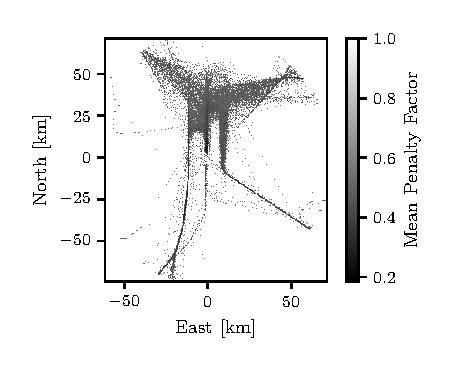
\includegraphics[width=\columnwidth]{figs/penalty}
  \caption{
    A heatmap showing the mean penalty factor across the $x$ and $y$
    axes of the configuration space.
    The $x$-axis represents the $x$ position in kilometers of each state with
    respect to \ac{sea} using the \ac{enu} convention.
    The $y$-axis represents the $y$ position in kilometers of each state with
    respect to \ac{sea} using the \ac{enu} convention.
  }
  \label{fig:penalty}
\end{figure}

I plot the penalty factor for each discretized state from a view
looking down the $z$ axis in Fig.~\ref{fig:penalty}.
I project the state space into \numprint{2} dimensions by taking the
mean of the penalty factor $J(\bar{s})$ over the $z$ and $\theta$
axes for each $x$ and $y$ coordinate.
The $x$ and $y$ axes are shown using the \ac{enu} convention.
The mean penalty factor is expressed as a grayscale color with lighter
coordinates indicating a higher value.
The darker lines in Fig.~\ref{fig:penalty} represent common routes
taken by human guided flights.

The approach I take to learn the penalty factor is different from the
approach presented in~\cite{tolstaya_rkk:planning_atc}.
Tolstaya et al. use maximum entropy inverse reinforcement learning
which updates the penalty according to gradient descent each time a
new solution is found by \ac{ara}.
Further, their penalty factor includes an inter-airplane safety cost
that extends their solution to handle multiple agents.
This approach seems out-of-scope for the research presented in this
paper, so my alternative formulation, which is completely offline, is
used instead.
I made heuristic comparisons with a figure from
\cite{tolstaya_rkk:planning_atc} that is similar to
Fig.~\ref{fig:penalty} that suggest our penalty factors are
comparable despite the differences in our approaches.

\section{DATASET PROCESSING} \label{sec:dataset}

I collect a dataset of human guided trajectories for benchmarking the
solutions returned by the planners and constructing the learned penalty factor.
The dataset contains real flight trajectories recorded during their landings at
\ac{sea} between January 11 and 14, 2016.
The raw data for each flight is downloaded from FlightAware.
The raw data consists of \ac{wgs} positions and heading measurements.
I process the raw data into a sequence of states which use the
Dubins airplane model.
For each trajectory, I compute the path length and the motion cost as
if they were solutions returned by a planner.

I start by pruning the start of each flight trajectory until it is
contained in the search space.
I define the search space using the great-circle distance with
reference to the \ac{wgs} position of \ac{sea}.
All positions outside a \numprint{75} kilometer great-circle
centered at \ac{sea} are excluded from the flight trajectory.
After pruning, I map the raw data from each trajectory into a
sequence of states.
The \ac{wgs} positions are converted to spatial coordinates using the
\ac{enu} convention.
The origin of the \ac{enu} reference frame is the \ac{wgs} center of \ac{sea}.
The headings in the raw data are consistent with the Dubins airplane model.
A state is constructed from each \ac{enu} position and heading.

The dataset is designed to follow the example provided
in the work by Tolstaya et al. with a few
differences~\cite{tolstaya_rkk:planning_atc}.
My dataset contains flights from January 14, 2016 which are not
included in the previous work.
The previous work does not discuss the size of their search space, so
I estimate it to be around \numprint{75} kilometers using their figures.

\section{EXPERIMENTAL DESIGN} \label{sec:exp_design}

I test four planner variants in my experiments and I explain their
configurations here.
For the two \ac{ara} variants, the only difference in their
configuration is their definition of cost-to-come.
\Ac{plara} uses a cost-to-come based on the \ac{pl} metric, but
\ac{mcara} uses a cost-to-come based on the \ac{mc} metric.
The two \ac{rrt} variants follow the same cost-to-come definitions as
their \ac{ara} counterparts, but they have more configuration differences.
The \ac{plrrt} planner uses a maximum edge length of \numprint{180}
seconds with a uniform sampling procedure.
The \ac{mcrrt} planner uses a maximum edge length of \numprint{30}
seconds with the distance-to-goal sampling procedure.

Each planner variant is tested on \numprint{1978} trials derived from
human guided trajectories.
A trial consists of a starting state and a goal state which
correspond to the first and last states in each human guided trajectory.
For each trial, I measure the number of iterations, the number of
states, and the cost of the best solution found.
For \ac{pl} and \ac{mc} variants the cost is the path length and
motion cost, respectively.
I record each metric at \numprint{30}, \numprint{60}, and
\numprint{180} seconds of runtime.
I measure \ac{ara} metrics each time the solution is improved, which
may not align with recording period, so recorded metrics correspond to
the best solution found at the time of recording.
The measuring approach for \ac{rrt} is more flexible as I can control
the exact number of iterations.
I record metrics after every \numprint{5000} iterations.
I execute trials on the \ac{hpc} cluster provided by \ac{cac}.
The trials are run on a machine with \numprint{64} cores and
\numprint{976} gigabytes of memory.
I allow trials to execute in parallel using the GNU Parallel
tool~\cite{tange:parallel}.

With the results collected from each trial, I compute five
statistical metrics for each planner variant.
I find the median number of iterations, the median number of expanded
states, the median cost, and the median cost margin for all planners.
For \ac{pl} and \ac{mc} variants, the cost and cost margin use the
path length and motion cost, respectively.
The cost margin is the difference between the cost of the planner
solution and the cost of the human trajectory for the same trial.
I also find the percent of trials, for each planner, which return a
solution.
All the statistical metrics are computed after each runtime period.

\section{RESULTS} \label{sec:results}

\begin{table*}[!t]
  \renewcommand{\arraystretch}{1.3}
  \caption{
    Experimental results from the ATC planning problem with \ac{ara}
    and \ac{rrt} variants.
  }
  \label{tab:results}
  \centering
  \begin{tabular}{llrrrrr}
    \hline
    \textbf{Planner} &
    \textbf{Runtime [s]} &
    \textbf{Median Iterations} &
    \textbf{Median States} &
    \textbf{Median Path Length} &
    \textbf{Median Cost Margin} &
    \textbf{\% Solved}  \\
    \hline

    \multirow[t]{3}{*}{\ac{plara}} & 30 & \numprint{213482.0} &
    \numprint{1038534.0} &
    \numprint{420.1} & \numprint{314.4} & \numprint{65.4} \\

    & 60 & \numprint{531878.0} &
    \numprint{2589844.0} & \numprint{363.1} & \numprint{254.5} &
    \numprint{82.1} \\

    & 180 & \numprint{1248564.0} & \numprint{5533595.0} &
    \numprint{320.7} & \numprint{211.4} & \numprint{96.1} \\

    \hline

    \multirow[t]{3}{*}{\ac{plrrt}} & 30 & \numprint{53000.0} &
    \numprint{47694.0} & \numprint{81.9}
    & \numprint{-31.0} & \numprint{100.0} \\

    & 60 & \numprint{79000.0} &
    \numprint{71092.0} & \numprint{81.9} & \numprint{-31.0} &
    \numprint{100.0} \\

    & 180 & \numprint{136000.0} & \numprint{122535.0} &
    \numprint{81.9} & \numprint{-31.0} & \numprint{100.0} \\

    \hline

    Human & & & & \numprint{111.3} & & \\

    \hline
    \textbf{Planner} &
    \textbf{Runtime [s]} &
    \textbf{Median Iterations} &
    \textbf{Median States} &
    \textbf{Median Motion Cost} &
    \textbf{Median Cost Margin} &
    \textbf{\% Solved}  \\
    \hline

    \multirow[t]{3}{*}{\ac{mcara}} & 30 & \numprint{0.0} &
    \numprint{0.0} & inf & inf & \numprint{25.8} \\

    & 60 & \numprint{0.0} & \numprint{0.0} & inf & inf & 44.3 \\

    & 180 & \numprint{2161474.0} & \numprint{9381285.0} &
    \numprint{735.8} & \numprint{629.1} & \numprint{79.8} \\

    \hline

    \multirow[t]{3}{*}{\ac{mcrrt}} & 30 & \numprint{365000.0} &
    \numprint{20392.5} & inf & inf & \numprint{0.0} \\

    & 60 & \numprint{635000.0} & \numprint{43617.0} & inf & inf &
    \numprint{0.1} \\

    & 180 & \numprint{1500000.0} & \numprint{150281.0} & inf & inf &
    \numprint{0.1} \\

    \hline
    Human & & & & \numprint{2322.0} & & \\
    \hline
  \end{tabular}
\end{table*}

My results indicate that \ac{ara} is better at finding solutions to the planning
problem than \ac{rrt}.
\Ac{ara} performs better in both the \ac{pl} and \ac{mc} variants of
the planning problem.
\Ac{rrt} fails to return a solution within the runtime limit in most
cases because it struggles with expanding states near the goal region.
In the following section, I present my experimental results and
I explain how I interpret my findings from them.

\begin{figure}[tbp]
  \includegraphics[width=\columnwidth]{figs/pl_cost_margin_ecdf}
  \caption{
    A plot of the empirical cummulative density function comparing
    the cost margin by path length of the \ac{plara} and \ac{plrrt} planners.
    The $x$-axis represents the cost margin by path length.
    The $y$-axis represents the probability that a solution has a certain
    cost margin based on the experimental results for all trials.
  }
  \label{fig:pl_cost_margins}
\end{figure}

Starting with the \ac{pl} variant of the planning problem, I consider
the cost margin by path length for \ac{plara} and \ac{plrrt} in
Fig.~\ref{fig:pl_cost_margins}.
Fig.~\ref{fig:pl_cost_margins} shows an empirical cummulative
distribution function for the cost margin by path length.
The $x$-axis shows values of the cost margin by path length and the
$y$-axis shows the cumulative probability of observing that cost margin.
The cost margins from solutions found by \ac{plara} are positive
which indicates that its solutions are consistently longer than the
human examples.
This is expected in part because the planner does not fully deflate $\epsilon$
within the runtime limit.
Conversely, \ac{plrrt} reports many negative cost margins.
The \numprint{0.8} quantile of \ac{plrrt} is \numprint{0} which
suggests that it frequently finds shorter trajectories than human examples.
These results are caused by the maximum edge length configured for \ac{plrrt}.

If the maximum edge length of \ac{rrt} puts the goal region within
the range of a single edge from the start state, then \ac{rrt}
collapses to returning the Dubins curve.
In \ac{plrrt} trials, the maximum edge length is equivalent to
\numprint{180} seconds of travel time which puts the goal region in
range for most trials.
The effect of this parameter is shown in Tab.~\ref{tab:results} where
the median path length does not improve with additional runtime and it
has a negative cost margin.
The median path length does not improve with additional runtime
because it finds the absolute shortest possible path on the first
iteration that the goal state is sampled.
The negative cost margin indicates that the solution returned by
\ac{plrrt} is shorter than the human guided trajectory.
The results show a negative cost margin because the \ac{plrrt} path is
always the absolute shortest possible path that obeys the kinodynamic
constraints of the airplane.
The shortest possible path is often not feasible in practical
scenarios where additional safety and higher order kinodynamic
constraints are present.
The Dubins airplane model does not encode these additional
constraints so the minimal path length solution is not always the best path.
Therefore, it is reasonable to consider reducing the maximum edge
length to prevent this case and force \ac{plrrt} to generate paths with
multiple intermediate states.

\begin{figure}[tbp]
  \centering
  \includegraphics[width=\columnwidth]{figs/rrt_search_trees}
  \caption{
    A trajectory plot comparing a solution found by \ac{plrrt} and
    the human guided reference.
    The goal region is denoted with a star.
    The plot axes are expressed using the \ac{enu} convention with
    the origin at \ac{sea}.
  }
  \label{fig:rrt_soln}
\end{figure}

In Fig.~\ref{fig:rrt_soln}, I compare the solution returned by
\ac{plrrt} to the human guided trajectory on a single flight from the dataset.
\Ac{plrrt} is given \numprint{3} minutes to find a solution.
Each state in trajectory is plotted as a colored circle and adjacent
circles are connected by a spline.
For the human guided trajectory, I plot the waypoints provided by the
flight tracking record.
I project each trajectory onto the $xy$-plane to give a better perspective.
In the human guided trajectory and \ac{plrrt} each state is
\numprint{30} seconds and \numprint{180} seconds apart, respectively.
The maximum edge length for \ac{plrrt} is oversized so its solutions
collapse to the Dubins curve.

When the maximum edge length is decreased, I notice that \ac{plrrt} can
no longer reach the goal reliably.
Since the size of the goal region is small compared to the size of the state
space, many samples explore unproductive regions and eat into runtime.
The complexity of the non-holonomic constraints impose an additional
penalty on the algorithm because more samples are required to
complete paths which are feasible by an aircraft.
Reaching the goal region is not a problem for \ac{ara} variants,
which indicates that the information provided by a heuristic may be
important in exploring efficiently.
\ac{plrrt} does not have access to heuristic information which may
contribute to the problem.
Further, the results in Tab.~\ref{tab:results} show that \ac{plrrt}
expands fewer states than \ac{ara} within the same runtime.
This means that \ac{plrrt} does not explore the search space as
throughly as \ac{ara}.
The smaller number of state expansions by \ac{plrrt} is likely due to the
overhead of computing the \ac{knn} because the Dubins curve needs to
be calculated for each of the candidate neighbors.

In the \ac{mc} variant of \ac{rrt}, I try to address the problem of
goal reachability by informing the sampling procedure using the
distance to the goal with the aim of increasing the efficiency of each
expanded state.
Unfortunately, even with a non-uniform sampling procedure, the
\ac{mcrrt} variant does not find the goal region reliably.
Tab.~\ref{tab:results} shows that only 0.1\% of \ac{mcrrt} trials
return a solution.
\Ac{mcrrt} still expands fewer states than \ac{mcara} which suggests
that the number of state expansions is still limiting the performance
of \ac{rrt}.
The lack of practical solutions from the \ac{rrt} variants make
comparison with \ac{ara} difficult.
As such, my results suggest that the implementations of \ac{rrt} that
I test here are insufficient for application to this planning problem.

Now, I consider the impact of the penalty factor on the solutions
returned by \ac{ara}.
I find that the introduction of the penalty factor reduces the
efficiency of the search.
In the results shown in Tab.~\ref{tab:results}, \ac{mcara} solves a
smaller fraction of trials than \ac{plara}, requires longer to find
an initial solution, has more iterations, and expands more states.
My result is different than the result obtained
in~\cite{tolstaya_rkk:planning_atc} where Tolstaya et al. see an increase in the
efficiency as their learning procedure converges.
I think that this is likely due to the differences in learning the
penalty factor.
It could be the case that \ac{mcara} is attempting to minimize the
penalty too much and is no longer guided by the heuristic.
The introduction of a tuning parameter on the importance of the
penalty may yield more efficient search with \ac{mcara}.

Despite the inefficient search, I find that the solutions returned by
\ac{mcara} follow the human guided trajectories more closely than \ac{plara}.
I can't make statistical claims about this result because I did not
record the \ac{pl} metric for solutions from \ac{mcara}.
Instead, I present a heuristic case in Fig.~\ref{fig:ara_sols} which shows
that \ac{mcara} returns a shorter solution than \ac{plara}.
The figure is formulated using the same method as Fig.~\ref{fig:rrt_soln}.
The \ac{mcara} trajectory mimics the descent pattern of the human
trajectory whereas the \ac{plara} trajectory descends very slowly in wide loops.
The trajectory returned by \ac{mcara} is also much more smooth.

\begin{figure}[tbp]
  \includegraphics[width=\columnwidth]{figs/ara_search_trees}
  \caption{
    A trajectory plot comparing a solution found by \ac{plara}, \ac{mcara},  and
    the human guided reference.
    The goal region is denoted with a star.
    The plot axes are expressed using the \ac{enu} convention with
    the origin at \ac{sea}.
  }
  \label{fig:ara_sols}
\end{figure}

\section{CONCLUSION} \label{sec:conclusion}

In this work, I implement and compare graph-based and sampling-based
planning algorithms for \ac{atc} using real flight
trajectories from \ac{sea}.
My results demonstrate that \ac{ara} consistently outperforms \ac{rrt}
in both finding solutions and achieving costs comparable to
human-guided trajectories.
The \ac{ara} variants successfully solve \numprint{96.1}\% and
\numprint{79.8}\% of trials for the \ac{pl} and \ac{mc} formulations,
respectively, within \numprint{180} seconds.
In contrast, \ac{rrt} variants struggle to reach the goal region
reliably, with \ac{mcrrt} solving only \numprint{0.1}\% of trials.

The poor performance of \ac{rrt} stems from two key factors.
First, the non-holonomic constraints of the Dubins airplane model
require careful trajectory planning, which increases the computational
overhead of the \ac{knn} calculations needed for rewiring.
Second, the small goal region relative to the large search space means
that uniform and weakly-informed sampling procedures spend significant
time exploring unproductive regions.
These findings suggest that heuristic information may be essential for
efficient exploration in planning problems with tight kinodynamic
constraints and small goal regions.

The learned penalty function successfully encodes common routes from
human-guided trajectories, as shown in Fig.~\ref{fig:penalty}.
However, the \ac{mcara} variant requires significantly more computation
time than \ac{plara} to find solutions, which indicates that the
current penalty formulation may be too conservative or that the
discretization is too fine.
Future work should explore alternative penalty learning methods that
better balance the trade-off between following human examples and
maintaining computational efficiency.

Future work should explore several directions to improve the
performance of automated \ac{atc} planning.
First, investigating adaptive or learned heuristics for \ac{rrt}
could help address the goal reachability problem by providing better
guidance toward feasible solutions.
Second, the penalty learning approach could be extended to incorporate
temporal information, such as time-of-day patterns or weather
conditions, which would better capture the dynamic nature of air
traffic control decisions.
Third, the current formulation assumes single-agent planning, but
realistic \ac{atc} requires coordinating multiple aircraft
simultaneously.
Extending these methods to handle multi-agent scenarios with
inter-airplane safety constraints would be an important step toward
practical deployment.
Finally, the discretization parameters for both the configuration
space and penalty factor should be optimized through systematic
parameter tuning, as the current choices significantly impact both
solution quality and computational efficiency.
Addressing these challenges would move automated \ac{atc} systems
closer to practical implementation.

\bibliographystyle{./IEEEtran}
\bibliography{./IEEEabrv.bib, ./references.bib}

\end{document}
